% ==============================================================================
% Chapter 4: Datasets, Evaluation Metrics, and Experimental Analysis (Clean Skeleton)
% Owners: TV1 (UniversalRAG), TV2 (ColPali & VisRAG), TV3 (Comparability & CoRe-MMRAG)
% Target length: ~7-9 pages
% ==============================================================================

\chapter{Dữ liệu, độ đo và phân tích kết quả thực nghiệm}
\label{chap:experiments}

\draftnote[Chung]{Chương 4 dài khoảng 7--9 trang. Không chép máy móc bảng số liệu thô: phải làm rõ điều kiện đánh giá, trả lời trực diện câu hỏi "các kết quả có so sánh trực tiếp được không?", và kiểm chứng xem thực nghiệm có thực sự chứng minh được tuyên bố của tác giả hay không.}

% ------------------------------------------------------------------------------
\section{Tổng quan bộ dữ liệu và benchmark đánh giá}
\label{sec:exp_datasets}

\draftnote[TV1 + TV2 + TV3]{Mỗi thành viên điền và phân tích nhóm benchmark thuộc phần mình phụ trách vào Bảng~\ref{tab:benchmarks}: ViDoRe 10 tác vụ Anh--Pháp (ColPali); 6 tập VQA + BEIR (VisRAG); 10 tập ID + 6 tập OOD (UniversalRAG); InfoSeek \& Encyclopedic-VQA (CoRe-MMRAG). Nêu rõ đặc điểm thống kê cơ bản cần thiết để hiểu và đối chiếu kết quả.}

\begin{table}[H]
\centering
\small
\caption[Tổng hợp các bộ dữ liệu và benchmark trọng tâm]{Tổng hợp các bộ dữ liệu và benchmark trọng tâm được sử dụng trong 4 nghiên cứu kỹ thuật.}
\label{tab:benchmarks}
\renewcommand{\arraystretch}{1.24}
\begin{tabularx}{\textwidth}{@{}P{3.1cm}P{2.5cm}P{2.3cm}L@{}}
\toprule
\rowcolor{tblhead}
\thead{Nhóm / Benchmark} & \thead{Bài báo} & \thead{Phương thức} & \thead{Đặc điểm nổi bật \& Thách thức} \\
\midrule
ViDoRe & ColPali & \dots & \dots \\
\rowcolor{zebrabg}
6 tập VQA + BEIR & VisRAG & \dots & \dots \\
10 tập ID + 6 tập OOD & UniversalRAG & Văn bản, bảng, ảnh, video & 7 lựa chọn định tuyến theo phương thức và mức độ chi tiết (10 tập ID chia 3:7; 6 tập OOD chỉ dùng kiểm thử); đánh giá cả truy xuất đơn kho và liên phương thức \cite{yeo2026universalrag} \\
\rowcolor{zebrabg}
InfoSeek \& Enc-VQA & CoRe-MMRAG & \dots & \dots \\
\bottomrule
\end{tabularx}
\end{table}

% TV1: Dataset and evaluation protocol breakdown for UniversalRAG
\paragraph{Hệ thống 16 bộ dữ liệu đa phương thức và nhiều mức độ chi tiết của UniversalRAG.}
Để đánh giá khả năng chọn đồng thời phương thức và mức độ chi tiết, UniversalRAG \cite{yeo2026universalrag} sử dụng 10 bộ dữ liệu cùng phân phối (\textit{in-domain} -- ID) và 6 bộ dữ liệu khác phân phối (\textit{out-of-domain} -- OOD) (Bảng~7 và Phụ lục~A của bài gốc). Mười tập ID được chia theo tỷ lệ 3:7 để huấn luyện bộ định tuyến và kiểm thử, bao phủ đủ 7 lựa chọn định tuyến:
\begin{itemize}
    \item \textit{Không cần truy xuất (None)}: MMLU gồm 1\,710 câu hỏi trắc nghiệm lấy từ tập \textit{dev}, dùng để kiểm tra xem hệ thống có tránh được bước truy xuất không cần thiết khi câu hỏi chỉ cần kiến thức phổ thông hay không.
    \item \textit{Văn bản ở hai mức độ chi tiết (Paragraph và Document)}: Natural Questions (NQ) gồm 2\,000 câu hỏi tra cứu một bước trên kho 850k đoạn Wikipedia (tối đa 100 từ, trung bình 100 token). HotpotQA gồm 2\,000 câu hỏi suy luận nhiều bước trên kho 509k tài liệu gộp liên quan (trung bình 693 token, nhiều mẫu dài trên 4k token theo cách ghép của LongRAG).
    \item \textit{Kết hợp văn bản và bảng (Paragraph+Table)}: HybridQA gồm 2\,000 câu hỏi với kho 15k mục. Khác với bản gốc vốn nối sẵn bảng Wikipedia với đoạn văn liên quan, nhóm tác giả tách chúng thành hai kho riêng để kiểm tra khả năng gọi đồng thời cả hai kho.
    \item \textit{Ảnh và kết hợp văn bản với ảnh}: MRAG-Bench gồm 1\,353 câu hỏi có kèm ảnh đầu vào trên kho 6k ảnh. WebQA gồm 2\,000 câu hỏi văn bản (đã lọc qua GPT-4o để bỏ các câu gắn cứng với một bức ảnh duy nhất) trên kho 20k đoạn văn và ảnh tách rời. InfoSeek gồm 2\,000 câu hỏi văn bản kèm ảnh từ tập \textit{dev} trên kho 20k đoạn văn và ảnh.
    \item \textit{Video ở hai mức độ chi tiết (Clip và Video)}: LVBench gồm 777 câu hỏi trên 89 video YouTube dài trung bình 3\,865 giây; phần lớn câu hỏi có mốc thời gian đáp án ngắn hơn 5 phút nên được xếp vào nhóm cần đoạn ngắn (Clip). Hai tập VideoRAG-Wiki và VideoRAG-Synth có 374 câu hỏi mỗi tập, dùng chung kho 9k video hướng dẫn HowTo100M dài trung bình 378 giây và đại diện cho nhóm cần xem toàn bộ video (Video).
\end{itemize}

Sáu tập OOD chỉ dùng ở bước kiểm thử mà không đưa vào huấn luyện bộ định tuyến, gồm: TruthfulQA (None, 790 câu trắc nghiệm), TriviaQA (Paragraph, 661 câu, kho 661k đoạn), SQuAD~v1.1 (Paragraph, 2\,000 câu, kho 1,19 triệu đoạn Wikipedia), 2WikiMultiHopQA (Document, 2\,000 câu, kho 12k tài liệu dài trung bình 562 token), Visual-RAG (Image, 374 câu hỏi văn bản tìm ảnh, kho 2k ảnh) và CinePile (Clip/Video, 1\,440 câu hỏi trên 144 video dài trung bình 158 giây).

Khi đọc số liệu của bài báo (Phụ lục~A.1--A.3 của \cite{yeo2026universalrag}), cần lưu ý hai chi tiết về cách chuẩn bị dữ liệu và tính điểm. Thứ nhất, hai tập LVBench và CinePile vốn là dữ liệu hỏi đáp trên một video cho sẵn chứ không phải bài toán tìm kiếm mở, nên nhóm tác giả đã dùng GPT-4o viết lại câu hỏi sang dạng văn bản độc lập dựa trên tiêu đề và thông tin kênh YouTube. Việc tách nhãn Clip/Video trên VideoRAG, CinePile cũng như bước lọc câu hỏi trên TriviaQA, WebQA đều do GPT-4o thực hiện. Thứ hai, mỗi nhóm tác vụ dùng độ đo riêng: \textit{Top-1 Accuracy} cho câu trắc nghiệm (MMLU, MRAG-Bench, LVBench, TruthfulQA, CinePile), \textit{Exact Match} (EM) và F1 cho câu trả lời ngắn (NQ, HotpotQA, HybridQA, TriviaQA, SQuAD, 2WikiMultiHopQA), độ chính xác theo quy ước gốc cho InfoSeek, và \textit{ROUGE-L} cùng \textit{BERTScore} cho câu trả lời dài tự do (WebQA, VideoRAG-Wiki/Synth, Visual-RAG). Điểm trung bình chung (Avg) được tính bằng cách lấy trung bình trong từng phương thức trước rồi mới lấy trung bình giữa các phương thức để các tập văn bản không chiếm trọng số quá lớn. Ngoài ra, toàn bộ kết quả được lấy từ một lần chạy duy nhất (\textit{single run}).

% ------------------------------------------------------------------------------
\section{Hệ thống độ đo đánh giá}
\label{sec:exp_metrics}

\draftnote[TV2]{Trình bày ngắn gọn định nghĩa, công thức chính và ý nghĩa khác biệt của 3 nhóm độ đo: (1) Truy xuất ($\mathrm{MRR}@K$, $\mathrm{nDCG}@K$, $\mathrm{Recall}@K$); (2) Tạo sinh \& Định tuyến ($\mathrm{EM}$, $\mathrm{Relaxed\ EM\ (\pm 5\%)}$, $\mathrm{VQA\ Accuracy}$, $\mathrm{BEM}$, $\mathrm{Routing\ Accuracy}$); (3) Hiệu năng hệ thống (Offline Indexing Latency, Online Query Latency, Storage Footprint KB/page).}

% ------------------------------------------------------------------------------
\section{Phân tích tính khả so sánh và đối chiếu kết quả định lượng}
\label{sec:exp_results}

\subsection{Các kết quả có thể so sánh trực tiếp không?}
\label{subsec:comparability}

\draftnote[TV3]{Trả lời trực tiếp yêu cầu bài tập: (1) Chỉ có cặp \textbf{ColPali và VisRAG} đối chiếu trực tiếp được trên phân khúc truy xuất tài liệu trực quan (VisRAG báo cáo trực tiếp In-domain MRR@10 cùng đối chiếu tốc độ và bộ nhớ); (2) Không so sánh ngang hàng bằng 1 con số duy nhất giữa UniversalRAG, CoRe-MMRAG và ColPali/VisRAG do khác bộ dữ liệu, đơn vị truy xuất, backbone và độ đo; (3) Lưu ý điểm giao tập \texttt{InfoSeek} giữa UniversalRAG và CoRe-MMRAG khác thiết lập nên phải phân tích riêng điều kiện thực nghiệm.}

\subsection{Tổng hợp kết quả định lượng theo từng nhóm bài toán}
\label{subsec:quantitative_tables}

\draftnote[TV2]{Điền Bảng~\ref{tab:vision_vs_text_retrieval} (đối chiếu Vision-space ColPali, ColQwen2, VisRAG-Ret với TextRAG OCR/Captioning, SigLIP, BiPali, ColSigLIP kèm trích nguồn Bảng/Hình bài gốc). Đồng thời bổ sung thêm 1 bảng hoặc mục phân tích nhỏ cho: (a) End-to-End Generation của VisRAG (MiniCPM-V 2.6, GPT-4o, top-1/3/6/10, BEIR); (b) Ablation Study của ColPali (448 vs 224, OOD DocMatix, bỏ \texttt{<unused0>}, Token Pooling factor=3).}

\begin{table}[H]
\centering
\small
\caption[Đối chiếu hiệu năng truy xuất, tốc độ và dung lượng giữa Vision-space RAG và TextRAG]{Đối chiếu hiệu năng truy xuất, tốc độ và dung lượng lưu trữ giữa Vision-space RAG và TextRAG.}
\label{tab:vision_vs_text_retrieval}
\renewcommand{\arraystretch}{1.24}
\begin{tabularx}{\textwidth}{@{}L M{2.05cm} M{2.15cm} M{1.75cm} M{2.05cm}@{}}
\toprule
\rowcolor{tblhead}
\thead{Phương pháp} & \thead{ViDoRe\newline (nDCG@5)} & \thead{VisRAG ID\newline (MRR@10)} & \thead{Index /\newline trang} & \thead{Dung lượng /\newline trang} \\
\midrule
Baseline TextRAG / VLM & \dots & \dots & \dots & \dots \\
\rowcolor{zebrabg}
ColPali / ColQwen2 & \dots & \dots & \dots & \dots \\
VisRAG-Ret & \dots & \dots & \dots & \dots \\
\bottomrule
\end{tabularx}
\end{table}

% TV1: Quantitative analysis for UniversalRAG
\subsubsection{Kết quả định lượng của UniversalRAG trên các tập ID và OOD}
\label{subsubsec:universalrag_quant}

UniversalRAG được so sánh với 12 phương pháp cơ sở chia thành 4 nhóm (Mục~3.1 của \cite{yeo2026universalrag}): trả lời trực tiếp không truy xuất (Naïve), 6 hệ thống RAG cố định một kho đơn lẻ (ParagraphRAG, DocumentRAG, TableRAG, ImageRAG, ClipRAG, VideoRAG), 4 phương pháp đưa mọi dữ liệu vào chung một không gian vector (UniRAG, GME, $\mathrm{PE}_{\mathrm{core}}$, VLM2Vec-V2) và phương pháp lấy ngữ cảnh từ tất cả các kho cùng lúc (MultiRAG). Bảng~\ref{tab:universalrag_results} tổng hợp kết quả tạo sinh trên 10 tập ID khi dùng mô hình sinh Qwen3-VL-8B-Instruct.

\begin{table}[H]
\centering
\footnotesize
\caption[Kết quả tạo sinh của UniversalRAG trên 10 tập In-Domain]{Kết quả tạo sinh của UniversalRAG và các phương pháp đối chứng trên 10 tập In-Domain với mô hình sinh Qwen3-VL-8B-Instruct (Nguồn: Bảng~1 của \cite{yeo2026universalrag}). Cột Avg tính trung bình theo từng phương thức (đã tính cả VideoRAG-Wiki: Naïve 19,78; Qwen3-VL-2B 20,86; Oracle 20,89 theo ROUGE-L).}
\label{tab:universalrag_results}
\setlength{\tabcolsep}{2.7pt}
\renewcommand{\arraystretch}{1.18}
\begin{tabularx}{\textwidth}{@{}L *{10}{r}@{}}
\toprule
\rowcolor{tblhead}
\thead{Phương pháp} & \thead{MMLU} & \thead{NQ} & \thead{Hotpot} & \thead{Hybrid} & \thead{MRAG} & \thead{WebQA} & \thead{InfoS.} & \thead{LVB} & \thead{Vid-S} & \thead{Avg} \\
\rowcolor{tblhead}
 & \scriptsize{(Acc)} & \scriptsize{(EM)} & \scriptsize{(EM)} & \scriptsize{(EM)} & \scriptsize{(Acc)} & \scriptsize{(R-L)} & \scriptsize{(Acc)} & \scriptsize{(Acc)} & \scriptsize{(R-L)} & \\
\midrule
Naïve (Không truy xuất) & 74,39 & 18,85 & 21,10 & 2,80 & 49,22 & 58,12 & 18,10 & 28,83 & 35,86 & 35,59 \\
\midrule
\rowcolor{zebrabg}
ParagraphRAG & 74,39 & 39,25 & 23,40 & 5,10 & 46,71 & 51,70 & 19,75 & 24,07 & 32,86 & 37,26 \\
DocumentRAG & 71,29 & 21,95 & 26,35 & 3,75 & 43,68 & 45,57 & 16,80 & 15,70 & 31,18 & 32,26 \\
\rowcolor{zebrabg}
TableRAG & 72,51 & 11,80 & 16,45 & 9,65 & 43,39 & 44,75 & 9,15 & 16,47 & 30,67 & 29,45 \\
ImageRAG & 73,33 & 17,15 & 19,15 & 2,20 & 52,55 & 67,96 & 20,15 & 25,35 & 36,10 & 35,04 \\
\rowcolor{zebrabg}
ClipRAG & 73,33 & 16,70 & 19,30 & 2,35 & 48,93 & 65,68 & 9,85 & 33,72 & 39,39 & 35,18 \\
VideoRAG & 74,91 & 15,85 & 20,00 & 2,30 & 48,04 & 64,97 & 11,25 & 32,05 & 40,05 & 35,01 \\
\midrule
\rowcolor{zebrabg}
UniRAG (Unified) & 70,06 & 19,30 & 19,35 & 2,85 & 44,86 & 53,26 & 19,05 & 22,65 & 32,41 & 32,93 \\
GME (Unified) & 70,41 & 20,05 & 19,50 & 3,00 & 49,45 & 55,03 & 19,20 & 23,68 & 33,02 & 33,88 \\
\rowcolor{zebrabg}
$\mathrm{PE}_{\mathrm{core}}$ (Unified) & 72,11 & 19,65 & 19,00 & 3,05 & 49,15 & 54,79 & 19,10 & 23,04 & 32,75 & 33,86 \\
VLM2Vec-V2 (Unified) & 71,70 & 19,95 & 18,50 & 2,95 & 46,78 & 52,35 & 18,80 & 23,55 & 33,38 & 33,31 \\
\rowcolor{zebrabg}
MultiRAG (All corpora) & 70,82 & 20,90 & 22,65 & 4,35 & 45,01 & 56,73 & 19,05 & 23,55 & 34,24 & 34,07 \\
\midrule
URAG (Qwen3-VL-2B) & 74,39 & 38,65 & \textbf{26,10} & \textbf{11,05} & \textbf{52,55} & \textbf{70,22} & 23,20 & \textbf{33,72} & \textbf{39,95} & \textbf{42,40} \\
\rowcolor{zebrabg}
URAG (InternVL3.5-1B) & 74,39 & \textbf{38,70} & 25,85 & 10,25 & \textbf{52,55} & 69,14 & \textbf{23,35} & \textbf{33,72} & 39,90 & 42,12 \\
URAG (T5Gemma 2 270M) & \textbf{74,62} & 38,65 & 25,90 & 9,95 & 50,33 & 69,03 & 21,95 & 33,59 & 39,43 & 41,68 \\
\rowcolor{zebrabg}
URAG (GPT-5, \textit{free}) & 74,27 & 34,50 & 24,35 & 4,95 & 50,11 & 62,38 & 21,45 & 32,30 & 35,94 & 39,26 \\
URAG (Qwen3-VL-8B, \textit{free}) & 74,09 & 35,20 & 24,65 & 5,25 & 50,04 & 65,27 & 20,65 & 32,43 & 34,77 & 39,46 \\
\midrule
\rowcolor{zebrabg}
Oracle (Cận trên) & 74,39 & 39,25 & 26,35 & 10,55 & 52,55 & 71,17 & 23,35 & 33,72 & 40,05 & 42,45 \\
\bottomrule
\end{tabularx}
\end{table}

Từ Bảng~\ref{tab:universalrag_results} có thể rút ra bốn nhận xét chính. Thứ nhất, các hệ thống RAG cố định một kho chỉ đạt kết quả tốt trên đúng tập dữ liệu khớp với phương thức và mức độ chi tiết của kho đó (ParagraphRAG đạt 39,25 EM trên NQ; DocumentRAG đạt 26,35 EM trên HotpotQA; ClipRAG đạt 33,72 Acc trên LVBench). Khi sang các tập khác loại, kết quả giảm mạnh do ngữ cảnh đưa vào không liên quan: ví dụ trên LVBench, ParagraphRAG chỉ đạt 24,07 so với 28,83 khi không truy xuất (Naïve), còn TableRAG kéo điểm trung bình chung xuống còn 29,45. Thứ hai, cả bốn phương pháp dùng chung không gian vector (UniRAG 32,93; GME 33,88; $\mathrm{PE}_{\mathrm{core}}$ 33,86; VLM2Vec-V2 33,31) lẫn MultiRAG (34,07) đều có điểm trung bình \textit{thấp hơn} cả mức không truy xuất Naïve (35,59). Điều này cho thấy việc lấy nhầm văn bản do khoảng cách phương thức hoặc nhồi cùng lúc dữ liệu từ mọi kho đều gây nhiễu cho mô hình sinh. Thứ ba, các biến thể bộ định tuyến có huấn luyện của UniversalRAG tiến rất sát cận trên Oracle (42,40 so với 42,45 ở Qwen3-VL-2B; biến thể nhỏ T5Gemma~2 270M cũng đạt 41,68). Riêng trên HybridQA, Qwen3-VL-2B đạt 11,05 EM, cao hơn nhẹ so với Oracle gán cứng theo tập (10,55 EM) nhờ bỏ bớt được nguồn không cần thiết ở một số câu hỏi đơn lẻ. Thứ tư, kết quả này lặp lại nhất quán trên hai mô hình sinh LVLM khác (Bảng~8 của \cite{yeo2026universalrag}): với InternVL3.5-8B, UniversalRAG (Qwen3-VL-2B) đạt trung bình 39,60 (so với Oracle 39,80, mức đơn kho cao nhất là ImageRAG 32,29, Naïve 31,29 và nhóm không gian vector chung 28,38--28,60); với Molmo2-4B, điểm đạt 41,83 (so với Oracle 42,05, ParagraphRAG 36,52, Naïve 33,19 và nhóm không gian vector chung 32,04--32,50).

\paragraph{Đánh giá vai trò của định tuyến phương thức, truy xuất liên phương thức và mức độ chi tiết.}
Bảng~\ref{tab:universalrag_routing_recall} trích dẫn độ chính xác chọn nhóm phương thức (\textit{Modality Accuracy} tính trên 4 nhóm lớn) cùng độ phủ truy xuất (\textit{Recall}@1/3/5). Song song đó, Hình~\ref{fig:tv1_universalrag_analysis} thể hiện tỷ lệ phân bổ phương thức thực tế, độ trễ truy vấn theo kích thước kho và ảnh hưởng của số tham số bộ định tuyến.

\begin{table}[H]
\centering
\small
\caption[Độ chính xác chọn phương thức và Recall của UniversalRAG so với nhóm không gian vector chung]{Độ chính xác chọn phương thức (\textit{Modality Acc}, \%) và độ phủ truy xuất (\textit{Recall}@1/3/5, \%) của nhóm không gian vector chung và UniversalRAG (Nguồn: Bảng~3 của \cite{yeo2026universalrag}).}
\label{tab:universalrag_routing_recall}
\renewcommand{\arraystretch}{1.20}
\begin{tabularx}{\textwidth}{@{}L *{4}{M{2.0cm}}@{}}
\toprule
\rowcolor{tblhead}
\thead{Phương pháp} & \thead{Modality Acc} & \thead{R@1} & \thead{R@3} & \thead{R@5} \\
\midrule
UniRAG (Unified) & 25,00 & 0,01 & 0,03 & 0,04 \\
\rowcolor{zebrabg}
GME (Unified) & 36,27 & 13,84 & 17,79 & 22,16 \\
$\mathrm{PE}_{\mathrm{core}}$ (Unified) & 25,00 & 0,67 & 1,20 & 1,85 \\
\rowcolor{zebrabg}
VLM2Vec-V2 (Unified) & 25,00 & 2,30 & 3,69 & 4,12 \\
\midrule
UniversalRAG (Qwen3-VL-2B, \textit{trained}) & \textbf{95,28} & \textbf{21,38} & \textbf{36,29} & \textbf{44,82} \\
\rowcolor{zebrabg}
UniversalRAG (InternVL3.5-1B, \textit{trained}) & 92,39 & 19,66 & 31,82 & 39,20 \\
UniversalRAG (GPT-5, \textit{training-free}) & 68,22 & 16,33 & 23,72 & 31,41 \\
\bottomrule
\end{tabularx}
\end{table}

Trong Bảng~\ref{tab:universalrag_routing_recall}, ba phương pháp UniRAG, $\mathrm{PE}_{\mathrm{core}}$ và VLM2Vec-V2 chỉ đạt đúng 25,00\% \textit{Modality Acc}, tức tương đương với việc luôn trả về một phương thức cố định duy nhất. Biểu đồ trên Hình~\ref{fig:tv1_universalrag_analysis}a (thống kê trên 200 câu hỏi mẫu mỗi tập) giải thích trực tiếp con số này: VLM2Vec-V2 lấy 100\% văn bản, GME lấy tới 85\% văn bản (chỉ có 12\% ảnh và 3\% video), trong khi UniversalRAG chia đều giữa không truy xuất (23\%), văn bản (30\%), ảnh (24\%) và video (23%), rất gần phân bố chuẩn 25\% của Oracle. Nhờ tìm đúng kho dữ liệu ngay từ đầu, UniversalRAG (Qwen3-VL-2B) nâng \textit{Recall}@5 lên 44,82\%, cao gấp đôi phương pháp tốt nhất trong nhóm dùng chung không gian vector là GME (22,16\%).

Hai thí nghiệm đánh giá từng thành phần tiếp theo làm rõ tác dụng của truy xuất liên phương thức và chọn mức độ chi tiết:
\begin{itemize}
    \item \textit{Truy xuất liên phương thức so với đơn phương thức (Bảng~2 của \cite{yeo2026universalrag})}: Khi cho phép bộ định tuyến chọn nhiều kho cùng lúc thay vì giới hạn ở một kho duy nhất, kết quả trên HybridQA và WebQA đều tăng ở cả ba bộ định tuyến. Cụ thể, Qwen3-VL-2B tăng từ 9,60 lên 11,05 EM (F1 từ 14,56 lên 16,23) trên HybridQA và từ 67,93 lên 70,22 ROUGE-L trên WebQA; InternVL3.5-1B tăng từ 9,65 lên 10,25 EM và từ 67,90 lên 69,14 ROUGE-L; GPT-5 tăng từ 4,75 lên 4,95 EM và từ 60,54 lên 62,38 ROUGE-L.
    \item \textit{Tác dụng của việc chia mức độ chi tiết (Bảng~4 và Bảng~9 của \cite{yeo2026universalrag})}: Với nhóm bộ định tuyến có huấn luyện (Bảng~9), việc phân biệt mức độ chi tiết giúp Qwen3-VL-2B tăng trên HotpotQA từ 22,25 lên 26,10 EM (F1 từ 30,38 lên 34,61) và trên LVBench từ 32,05 lên 33,72 Acc; mức tăng tương tự cũng xuất hiện ở InternVL3.5-1B (23,00 lên 25,85 EM; 32,05 lên 33,72 Acc) và T5Gemma~2 270M (22,55 lên 25,90 EM; 31,40 lên 33,59 Acc). Với nhóm bộ định tuyến dùng prompt khi tăng số mức chi tiết $\#\mathrm{Gn}$ từ 1 lên 4 (Bảng~4, thêm các mức trung gian \textit{Passage}, \textit{Section} và \textit{Sequence}, \textit{Segment}), Qwen3-VL-8B tăng đều từ 23,85 lên 25,05 EM trên HotpotQA và từ 31,53 lên 33,20 Acc trên LVBench; còn GPT-5 tăng từ 23,20 lên 24,70 EM (có giảm nhẹ từ 24,35 xuống 24,20 ở mức $\#\mathrm{Gn}=3$) và từ 31,92 lên 32,85 Acc.
\end{itemize}

\begin{figure}[H]
\centering
\begin{subfigure}[t]{0.32\textwidth}
    \centering
    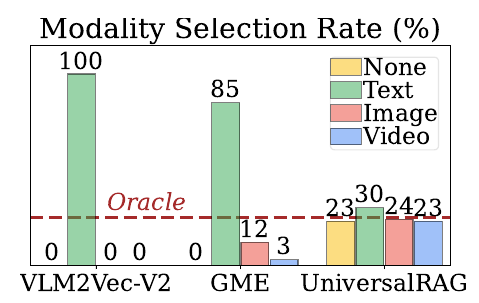
\includegraphics[width=\linewidth]{figures/tv1/universalrag-modality-dist.png}
    \caption{Tỷ lệ phương thức truy xuất (Hình~4 gốc).}
    \label{fig:tv1_modality_dist}
\end{subfigure}
\hfill
\begin{subfigure}[t]{0.32\textwidth}
    \centering
    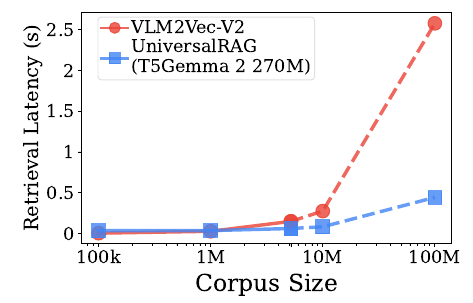
\includegraphics[width=\linewidth]{figures/tv1/universalrag-latency.png}
    \caption{Độ trễ theo quy mô kho (Hình~5 gốc).}
    \label{fig:tv1_latency}
\end{subfigure}
\hfill
\begin{subfigure}[t]{0.32\textwidth}
    \centering
    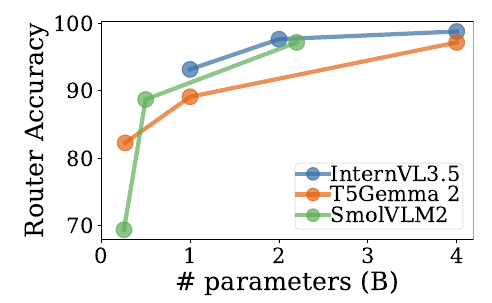
\includegraphics[width=\linewidth]{figures/tv1/universalrag-router-size.png}
    \caption{Độ chính xác theo cỡ router (Hình~6 gốc).}
    \label{fig:tv1_router_size}
\end{subfigure}
\caption[Phân tích tỷ lệ chọn phương thức, độ trễ truy vấn và kích thước bộ định tuyến của UniversalRAG]{Ba kết quả phân tích bổ sung của UniversalRAG \cite{yeo2026universalrag}: (a) tỷ lệ các phương thức được lấy ra trên 200 truy vấn mẫu mỗi tập; (b) thời gian truy xuất trung bình mỗi câu hỏi khi tăng quy mô kho từ 100k lên 100M mục (dùng router T5Gemma~2 270M); và (c) độ chính xác phân loại khi thay đổi kích thước router từ 256M đến 4B tham số.}
\label{fig:tv1_universalrag_analysis}
\end{figure}

Về tốc độ truy vấn, Hình~\ref{fig:tv1_universalrag_analysis}b kiểm chứng trực tiếp Mệnh đề~C.4: ở quy mô nhỏ (100k--1M mục), thời gian chạy bộ định tuyến $C$ làm cho UniversalRAG chậm tương đương hoặc nhỉnh hơn chút ít so với tìm trực tiếp. Tuy nhiên, khi tổng số mục tăng qua ngưỡng 10M lên tới 100M, độ trễ tìm kiếm trên kho gộp chung của VLM2Vec-V2 vọt lên gần 2,5 giây mỗi câu hỏi, trong khi UniversalRAG (dùng T5Gemma~2 270M) tăng chậm hơn nhiều nhờ chỉ phải tìm trên kho con đã chọn. Bên cạnh đó, Hình~\ref{fig:tv1_universalrag_analysis}c cho thấy độ chính xác định tuyến tăng theo số lượng tham số trên cả ba dòng mô hình (InternVL3.5, T5Gemma~2, SmolVLM2), nhưng ngay ở mốc 1B tham số đã đạt khoảng 90\%, đủ nhẹ để dùng làm bước tiền xử lý.

\paragraph{Khả năng tổng quát hóa trên dữ liệu ngoài phân phối (OOD) và kết hợp bộ định tuyến.}
Bảng~\ref{tab:universalrag_ood_ensemble} so sánh độ chính xác định tuyến trên cả 7 nhánh (\textit{Router Acc}, phân biệt với \textit{Modality Acc} 4 nhóm ở Bảng~\ref{tab:universalrag_routing_recall}) cùng điểm tạo sinh trung bình giữa 10 tập ID và 6 tập OOD.

\begin{table}[H]
\centering
\small
\caption[So sánh kết quả In-Domain và Out-of-Domain của UniversalRAG và các phương án kết hợp]{Độ chính xác định tuyến 7 nhánh (\textit{Router Acc}, \%) và điểm tạo sinh trung bình (Avg) trên 10 tập In-Domain và 6 tập Out-of-Domain với Qwen3-VL-8B-Instruct (Nguồn: Bảng~5 và Bảng~10 của \cite{yeo2026universalrag}).}
\label{tab:universalrag_ood_ensemble}
\renewcommand{\arraystretch}{1.20}
\begin{tabularx}{\textwidth}{@{}L *{4}{M{1.95cm}}@{}}
\toprule
\rowcolor{tblhead}
\thead{Phương pháp} & \thead{ID Router Acc} & \thead{ID Avg} & \thead{OOD Router Acc} & \thead{OOD Avg} \\
\midrule
Random (Chọn ngẫu nhiên 7 nhánh) & 14,29 & 31,75 & 14,29 & 37,85 \\
\rowcolor{zebrabg}
ParagraphRAG (Tốt nhất đơn kho, Bảng~10) & -- & 37,26 & -- & 42,62 \\
GME (Unified, Bảng~10) & -- & 33,88 & -- & 39,22 \\
\rowcolor{zebrabg}
$\mathrm{PE}_{\mathrm{core}}$ (Unified) & -- & 33,86 & -- & 39,08 \\
VLM2Vec-V2 (Unified) & -- & 33,31 & -- & 38,99 \\
\rowcolor{zebrabg}
MultiRAG (All corpora, Bảng~10) & -- & 34,07 & -- & 39,15 \\
\midrule
URAG (Qwen3-VL-2B, \textit{trained}) & 95,81 & 42,40 & 71,29 & 44,07 \\
\rowcolor{zebrabg}
URAG (InternVL3.5-1B, \textit{trained}) & 93,16 & 42,12 & 67,85 & 43,80 \\
URAG (T5Gemma 2 270M, \textit{trained}, Bảng~10) & -- & 41,68 & -- & 43,61 \\
\rowcolor{zebrabg}
URAG (GPT-5, \textit{training-free})$^{(*)}$ & 72,33 & 39,26 & 77,38 & 44,39 \\
URAG (Qwen3-VL-8B, \textit{training-free}, Bảng~10) & -- & 39,46 & -- & 44,35 \\
\midrule
\rowcolor{zebrabg}
Ensemble (Confidence-based) & 96,02 & 42,53 & \textbf{80,71} & \textbf{44,71} \\
Ensemble (Majority Voting) & \textbf{98,33} & \textbf{42,83} & 78,56 & 44,54 \\
\midrule
\rowcolor{zebrabg}
Oracle (Cận trên, Bảng~10) & -- & 42,45 & -- & 46,24 \\
\bottomrule
\end{tabularx}
\par\vspace{4pt}
{\footnotesize\raggedright\textit{Ghi chú:} $^{(*)}$ Trong bài báo gốc \cite{yeo2026universalrag}, điểm ID Avg của UniversalRAG (GPT-5) ghi là 39,26 ở Bảng~1 nhưng lại in là 41,68 ở Bảng~5; bảng trên giữ con số 39,26 khớp với các cột thành phần của Bảng~1 và nêu rõ điểm lệch này tại Mục~\ref{sec:exp_critique}.\par}
\end{table}

Số liệu ở Bảng~\ref{tab:universalrag_ood_ensemble} cho thấy sự khác biệt rõ giữa hai hướng thiết kế bộ định tuyến khi đổi miền dữ liệu. Trên 6 tập OOD chưa từng gặp lúc huấn luyện, độ chính xác định tuyến của Qwen3-VL-2B giảm 24,52 điểm phần trăm (từ 95,81\% xuống 71,29%), còn InternVL3.5-1B giảm 25,31 điểm (từ 93,16\% xuống 67,85%). Trái lại, bộ định tuyến dùng prompt GPT-5 không bị phụ thuộc vào phân phối huấn luyện nên đạt 77,38\% \textit{Router Acc} và 44,39 Avg trên OOD, vượt qua tất cả các bộ định tuyến đơn lẻ có huấn luyện (biến thể dùng prompt Qwen3-VL-8B cũng đạt tới 44,35 Avg ở Bảng~10). Khi ghép hai loại lại, phương án \textit{Confidence-based Ensemble} đạt kết quả OOD cao nhất với 80,71\% \textit{Router Acc} và 44,71 Avg (vượt mức tốt nhất của các baseline là ParagraphRAG 42,62 hay GME 39,22, tiến gần hơn tới Oracle 46,24), còn \textit{Majority Voting} đạt mức cao nhất trên ID với 98,33\% \textit{Router Acc} và 42,83 Avg.

\draftnote[TV3]{Tra cứu trực tiếp bản PDF gốc \textit{CoRe-MMRAG} (\texttt{2025.acl-long.1583}) để điền đầy đủ số liệu chính xác vào Bảng~\ref{tab:core_results}, ghi rõ tên MLLM nền và các baseline giải xung đột liên quan.}

\begin{table}[H]
\centering
\small
\caption[Kết quả thực nghiệm của CoRe-MMRAG trên các benchmark KB-VQA]{Kết quả thực nghiệm của CoRe-MMRAG trên các benchmark KB-VQA.}
\label{tab:core_results}
\renewcommand{\arraystretch}{1.24}
\begin{tabularx}{\textwidth}{@{}P{4.2cm}M{2.2cm}M{2.6cm}L@{}}
\toprule
\rowcolor{tblhead}
\thead{Phương pháp đối chứng} & \thead{InfoSeek} & \thead{Enc-VQA} & \thead{Ghi chú thiết lập} \\
\midrule
MLLM nền (No-RAG) & \dots & \dots & \dots \\
\rowcolor{zebrabg}
Standard Multimodal RAG & \dots & \dots & \dots \\
CoRe-MMRAG & \dots & \dots & \dots \\
\bottomrule
\end{tabularx}
\end{table}

% ------------------------------------------------------------------------------
\section{Kiểm chứng lập luận tác giả và đánh giá phản biện của nhóm}
\label{sec:exp_critique}

\draftnote[TV1 + TV2 + TV3]{Trả lời trực tiếp câu hỏi: ``Kết quả thực nghiệm có hỗ trợ những ưu điểm mà tác giả đưa ra không?'' và chỉ ra điểm yếu/đánh đổi ẩn ở từng bài:
(1) \textbf{ColPali}: Sụt mạnh ở 224$\times$224 (-24.8 điểm); Token Pooling giảm chất lượng trên trang chữ dày (\textit{Shift}); chưa đánh giá tạo sinh đầu--cuối; kiểm tra lại PDF gốc hai điểm lệch giữa văn bản Mục 6 và Bảng 7 (số patch ở 224$\times$224 và chiều biến thiên của \textit{No Q.A. Tokens} trên tiếng Pháp).
(2) \textbf{VisRAG}: Hiệu năng tạo sinh giảm khi tăng từ top-3 xuống top-10 do nhiễu đa trang; thiếu chứng minh lý thuyết về giới hạn 1 vector đơn.
(3) \textbf{UniversalRAG}: Giả định toán học còn lý tưởng; độ chính xác định tuyến OOD giảm so với ID.
(4) \textbf{CoRe-MMRAG}: Đánh đổi độ trễ suy luận 4 bước và bị giới hạn bởi năng lực đọc ảnh của MLLM nền.}

% TV1: Critical verification of UniversalRAG's claims and limitations
\paragraph{Kiểm chứng lập luận và đánh giá phản biện đối với UniversalRAG.}
Khi đối chiếu các tuyên bố của tác giả trong \cite{yeo2026universalrag} với số liệu ở Mục~\ref{subsec:quantitative_tables}, có thể thấy thực nghiệm đã chứng minh được ba kết luận chính: (i) tách riêng kho theo từng phương thức giúp tránh được hiện tượng thiên lệch về văn bản của không gian biểu diễn chung (\textit{Modality Acc} tăng từ 25,00\%--36,27\% lên 95,28\%, \textit{Recall}@5 tăng gấp đôi lên 44,82\% ở Bảng~3 và tỷ lệ chọn phương thức cân bằng trên Hình~4); (ii) cả hai cơ chế truy xuất liên phương thức và phân tách mức độ chi tiết đều mang lại cải thiện trên nhiều bộ dữ liệu và cả ba mô hình sinh LVLM (Bảng~2, 4, 8 và 9); và (iii) lợi thế về tốc độ tìm kiếm thể hiện rõ khi tổng quy mô kho vượt qua mốc 10M mục (Hình~5). Dù vậy, khi xét kỹ điều kiện thí nghiệm, phương pháp này vẫn còn bốn hạn chế và đánh đổi cần lưu ý:

\begin{enumerate}
    \item \textit{Giả định toán học đơn giản hóa nhiều so với dữ liệu thực}: Chứng minh Mệnh đề~2.1 và Mệnh đề~C.1 (Phụ lục~C.1) giả thiết các biến điểm số $X_c$ độc lập nhau, có kỳ vọng bằng 0, cùng tuân theo phân phối \textit{sub-Gaussian} với phương sai $\sigma^2$ như nhau trên mọi kho, rồi chặn trên bằng bất đẳng thức hợp (\textit{union bound}). Trong dữ liệu thực, các tài liệu cùng chủ đề có điểm tương đồng tương quan chặt với nhau và phân bố mật độ giữa kho ảnh, bảng và văn bản rất khác nhau. Tương tự, Mệnh đề~C.4 giả sử các kho con có cùng kích thước $N$ và việc truy vấn song song nhiều kho không gây tranh chấp tài nguyên phần cứng.
    \item \textit{Độ chính xác định tuyến giảm mạnh trên tập OOD và phụ thuộc nhiều vào GPT-4o}: Khi sang 6 tập OOD, độ chính xác của các bộ định tuyến có huấn luyện giảm khoảng 25 điểm phần trăm (Bảng~5: Qwen3-VL-2B giảm từ 95,81\% xuống 71,29\%; InternVL3.5-1B giảm từ 93,16\% xuống 67,85\%). Nguyên nhân chính đã được nhóm tác giả nêu trong mục \textit{Limitations}: hiện chưa có tập dữ liệu nào do con người gán nhãn phương thức và mức độ chi tiết cho từng câu hỏi. Nhãn huấn luyện được lấy tự động theo nguồn dữ liệu đích của từng tập, còn ở nhiều tập kiểm thử (LVBench, CinePile, WebQA, TriviaQA, VideoRAG), câu hỏi hoặc nhãn mức độ chi tiết đều do GPT-4o viết lại, lọc bớt hoặc phân loại tự động (Phụ lục~A.1--A.2, Hình~10--11). Cách chuẩn bị dữ liệu như vậy có thể làm câu hỏi mang văn phong gần với mô hình ngôn ngữ lớn, gián tiếp có lợi cho bộ định tuyến dùng prompt.
    \item \textit{Chia quá nhiều mức chi tiết không phải lúc nào cũng tăng điểm và dễ nhầm ở vùng giáp ranh}: Trên HotpotQA với GPT-5 (Bảng~4), khi tăng số mức chi tiết $\#\mathrm{Gn}$ từ 2 lên 3 thì điểm EM giảm nhẹ từ 24,35 xuống 24,20 rồi mới tăng lại ở $\#\mathrm{Gn}=4$. Nguyên nhân là khi chia nhỏ thêm các mức \textit{Passage} và \textit{Section}, ranh giới định nghĩa giữa các mức gần nhau trở nên khó phân biệt hơn. Năm ví dụ lỗi tại Bảng~15 của bài gốc cũng cho thấy bộ định tuyến dễ nhầm ở các câu hỏi giáp ranh (chọn \textit{No} thay vì \textit{Paragraph} cho câu hỏi về nguồn gốc từ vựng, nhầm \textit{Clip} sang \textit{Image} hoặc \textit{Video}, và thiếu nhánh \textit{Image} khi câu hỏi cần \textit{Paragraph+Image}), bên cạnh việc phụ thuộc vào ngưỡng xác suất cố định 0,8 ở bước suy luận đa nhãn (Phụ lục~B).
    \item \textit{Chi phí xây dựng hệ thống đa chỉ mục và giới hạn của thiết kế thí nghiệm}: Để vận hành UniversalRAG, hệ thống phải lập và bảo trì đồng thời 6 chỉ mục riêng, nạp 3 bộ mã hóa khác nhau (Qwen3-Embedding-4B, VLM2Vec-V2 và biểu diễn vector đặc theo từng hàng của bảng), đồng thời chạy nhiều bước tiền xử lý ngoại tuyến như cắt cảnh video bằng PySceneDetect, lấy mẫu 32 khung hình và sinh mô tả ảnh, lời thoại video để tính điểm kết hợp theo tỷ lệ 0,8/0,2 (Phụ lục~B). Phần chi phí lưu trữ và tiền xử lý này không nằm trong phép đo thời gian truy vấn ở Hình~5. Ngoài ra, mọi con số thực nghiệm chỉ chạy một lần duy nhất (Phụ lục~A.3) nên không có độ lệch chuẩn để đánh giá mức dao động, và có một điểm không khớp nhỏ giữa Bảng~1 với Bảng~5 của bài gốc ở điểm trung bình ID của UniversalRAG (GPT-5) (Bảng~1 ghi 39,26 nhưng Bảng~5 ghi 41,68, trùng với điểm của T5Gemma~2 270M ở Bảng~1). Từ đó có thể thấy UniversalRAG phù hợp nhất khi kho dữ liệu thực sự lớn, trải trên nhiều phương thức và có dùng kết hợp bộ định tuyến (\textit{Ensemble}) để tránh sụt giảm khi gặp câu hỏi mới.
\end{enumerate}
